\documentclass[aspectratio=169]{beamer}
\usepackage{babel}
% \usepackage[german]{babel}

\usepackage{tikz, transparent, colortbl, listings, pgfplots}
\usepackage[export]{adjustbox}
\usepackage[skins,theorems]{tcolorbox}
\usepackage{graphicx}
\usepackage{color}

\usetikzlibrary{automata,positioning}
\setbeamercovered{transparent}
\pgfplotsset{compat=1.18}
\tcbset{highlight math style={enhanced,colframe=red,colback=white,arc=0pt,boxrule=1pt}}

%
% Cited from Ausarbeitung/aspdoc.cls
%
\lstset{
    language=C++,
    basicstyle=\upshape\footnotesize\ttfamily,
    numbers=left,                   % where to put the line-numbers
    numberstyle=\tiny\color{gray},  % the style that is used for the line-numbers
    numbersep=5pt,                  % how far the line-numbers are from the code
    showstringspaces=false,
    frame=single,                   % adds a frame around the code
    rulecolor=\color{black},
    tabsize=2,                      % sets default tabsize to 2 spaces
    captionpos=b,                   % sets the caption-position to bottom
    breaklines=true,                % sets automatic line breaking
    breakatwhitespace=false,        % sets if automatic breaks should only happen at whitespace
    title=\lstname,                 % show the filename of files included with \lstinputlisting;
    keywordstyle=\color{blue},      % keyword style
    commentstyle=\color{dkgreen},   % comment style
    stringstyle=\color{mauve},      % string literal style
    escapeinside={\%*}{*)},         % if you want to add LaTeX within your code
}

% \lstset{
%     language=YAML,
%     basicstyle=\upshape\footnotesize\ttfamily,
%     numbers=left,
%     numberstyle=\tiny\color{gray},
%     numbersep=5pt,
%     showstringspaces=false,
%     frame=single,
%     rulecolor=\color{black},
%     tabsize=2,
%     captionpos=b,
%     breaklines=true,
%     breakatwhitespace=false,
%     title=\lstname,
%     keywordstyle=\color{blue},
%     commentstyle=\color{dkgreen},
%     stringstyle=\color{mauve},
%     escapeinside={\%*}{*)},
% }

% Useful Read:
% https://www.overleaf.com/learn/latex/Beamer

\title{Molecular Dynamics}
\subtitle{Group A}
\author{Haoyuan Ma \and Zhengying Zhao \and Anatoly Weinstein}
\date{31st of October 2025}

\newcommand{\framebackground}[2]{
    \begin{tikzpicture}
    \transparent{#1}
    \node[inner sep=0] at (current page.center) {
        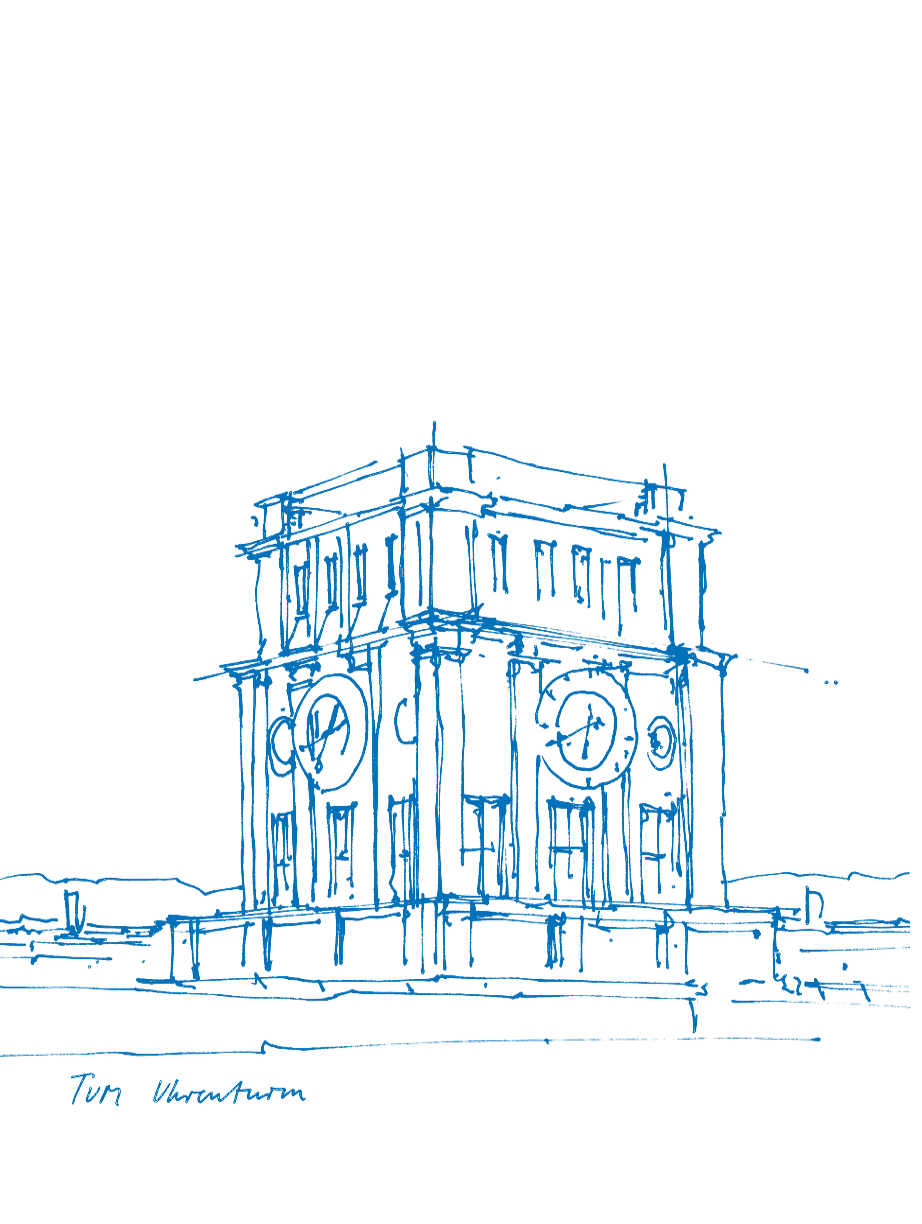
\includegraphics[height=\paperheight, right]{./media/tum-uhrenturm.png}
    };
    \transparent{1}
    \node[anchor=south, text width=\paperwidth, text height=1.5cm, draw=none, align=center] at (current page.south) {
        \insertpagenumber
    };
    \transparent{#2}
    \node[anchor=south, text width=\paperwidth, text height=1.5cm, draw=none, align=right] at (current page.south) {
        \small Haoyuan Ma, Zhengying Z, Anatoly W. \,\,
    };
    \end{tikzpicture}
}

\newcommand{\headerframe}{
    \usebackgroundtemplate{
        \framebackground{0.2}{1}
    }
}

\newcommand{\simpleframe}{
    \usebackgroundtemplate{
        \framebackground{0}{1}
    }
}

\newcommand{\blue}[1]{{\color{beamer@blendedblue} #1}}
\newcommand{\yellow}[1]{{\color[HTML]{AF8F10} #1}}
\newcommand{\gray}[1]{{\color[HTML]{8F8F8F} #1}}
\newcommand{\red}[1]{{\color[HTML]{FF5F5F} #1}}

\begin{document}

%
% Frame
%
    \usebackgroundtemplate{\framebackground{0.2}{0}}
    \begin{frame}
        \maketitle
    \end{frame}

    \simpleframe\begin{frame}{Thermostats}
                    \begin{center}
                        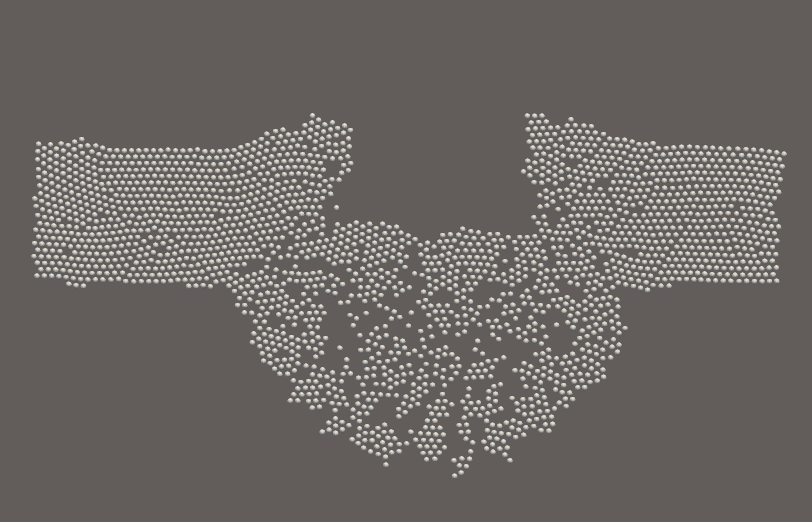
\includegraphics[width=0.6\textwidth]{media/lowTemp_2Bodies.png}
                    \end{center}
                    As seen in lowTemp2Bodies.mp4
    \end{frame}

    \simpleframe\begin{frame}{Thermostats}
                    \begin{center}
                        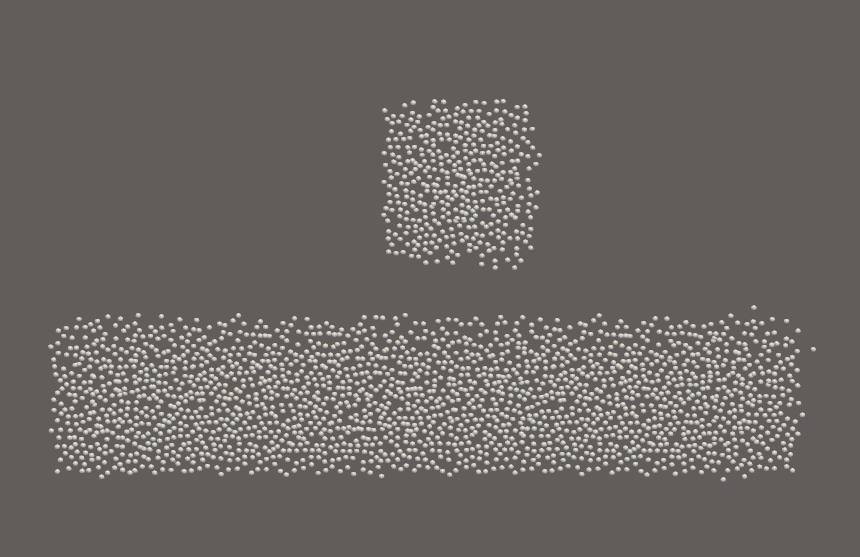
\includegraphics[width=0.6\textwidth]{media/highTemp_2Bodies.png}
                    \end{center}
                    As seen in highTemp2Bodies.mp4
    \end{frame}

    \simpleframe\begin{frame}{Problem with reflective boundaries}
                    \begin{center}
                        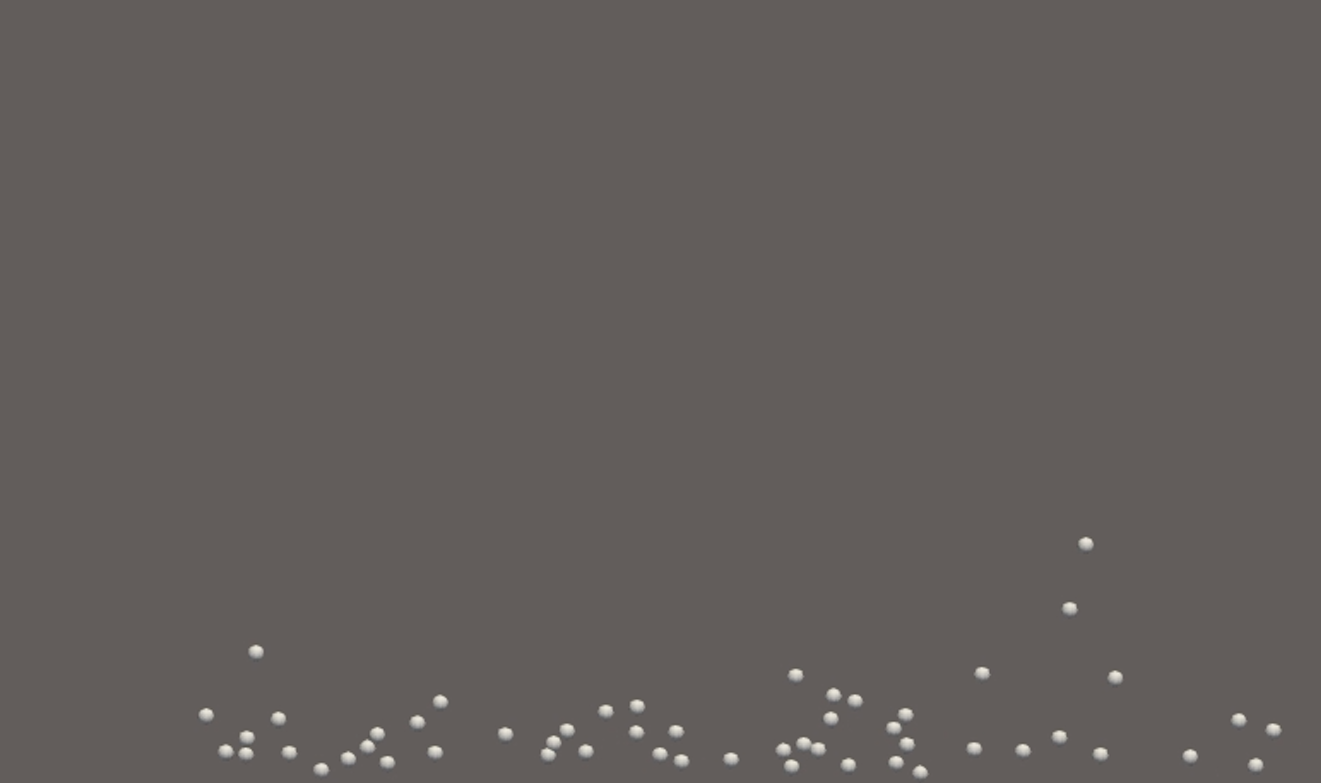
\includegraphics[width=0.60\textwidth]{media/normGrav.png}
                    \end{center}
                    A problem appears with balancing repulsion strength between wall and particles.

                    As seen in liquid2normGravity.mp4
    \end{frame}

    \simpleframe\begin{frame}{Problem with reflective boundaries}
                    \begin{center}
                        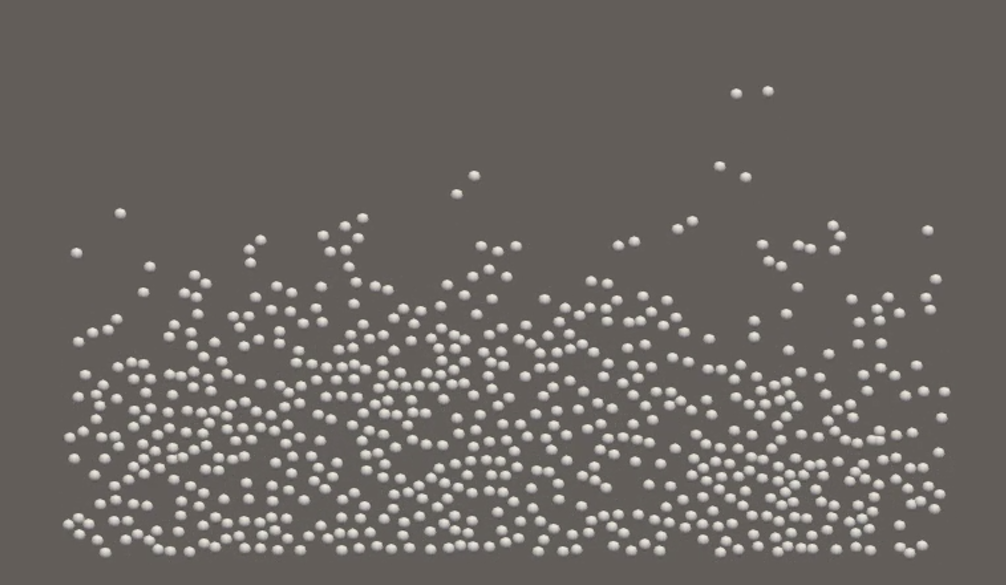
\includegraphics[width=0.60\textwidth]{media/lowGrav.png}
                    \end{center}
                    Solved by clamping particles back into domain space, resulting unnatural velocity behavior.
                    This is not ideal.
                    As seen in liquid2LowGravity.mp4
    \end{frame}

    \simpleframe\begin{frame}{Profiling Integration}
                    \begin{center}
                        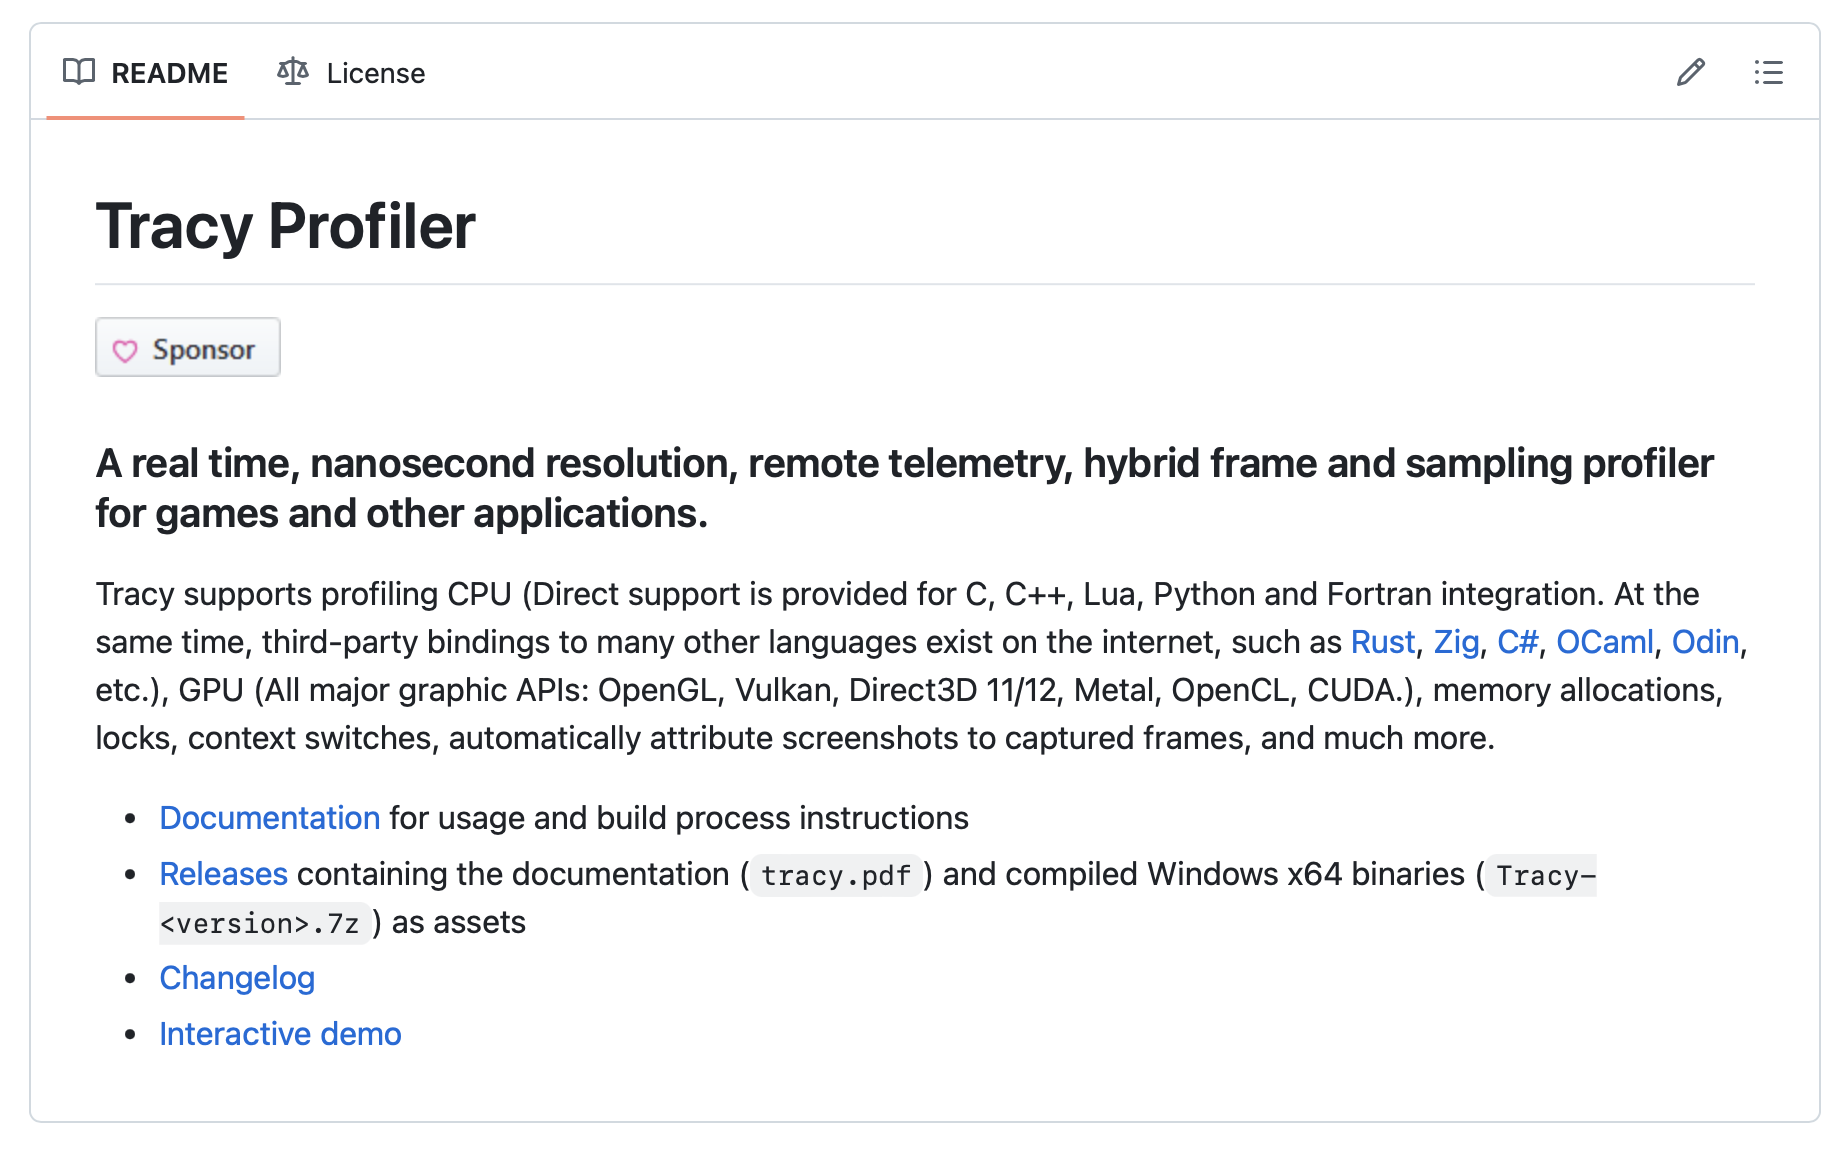
\includegraphics[width=0.85\textwidth]{media/profile-tracy.png}
                    \end{center}
    \end{frame}

    \simpleframe\begin{frame}{Profiling Integration}{Example}
                    \begin{center}
                        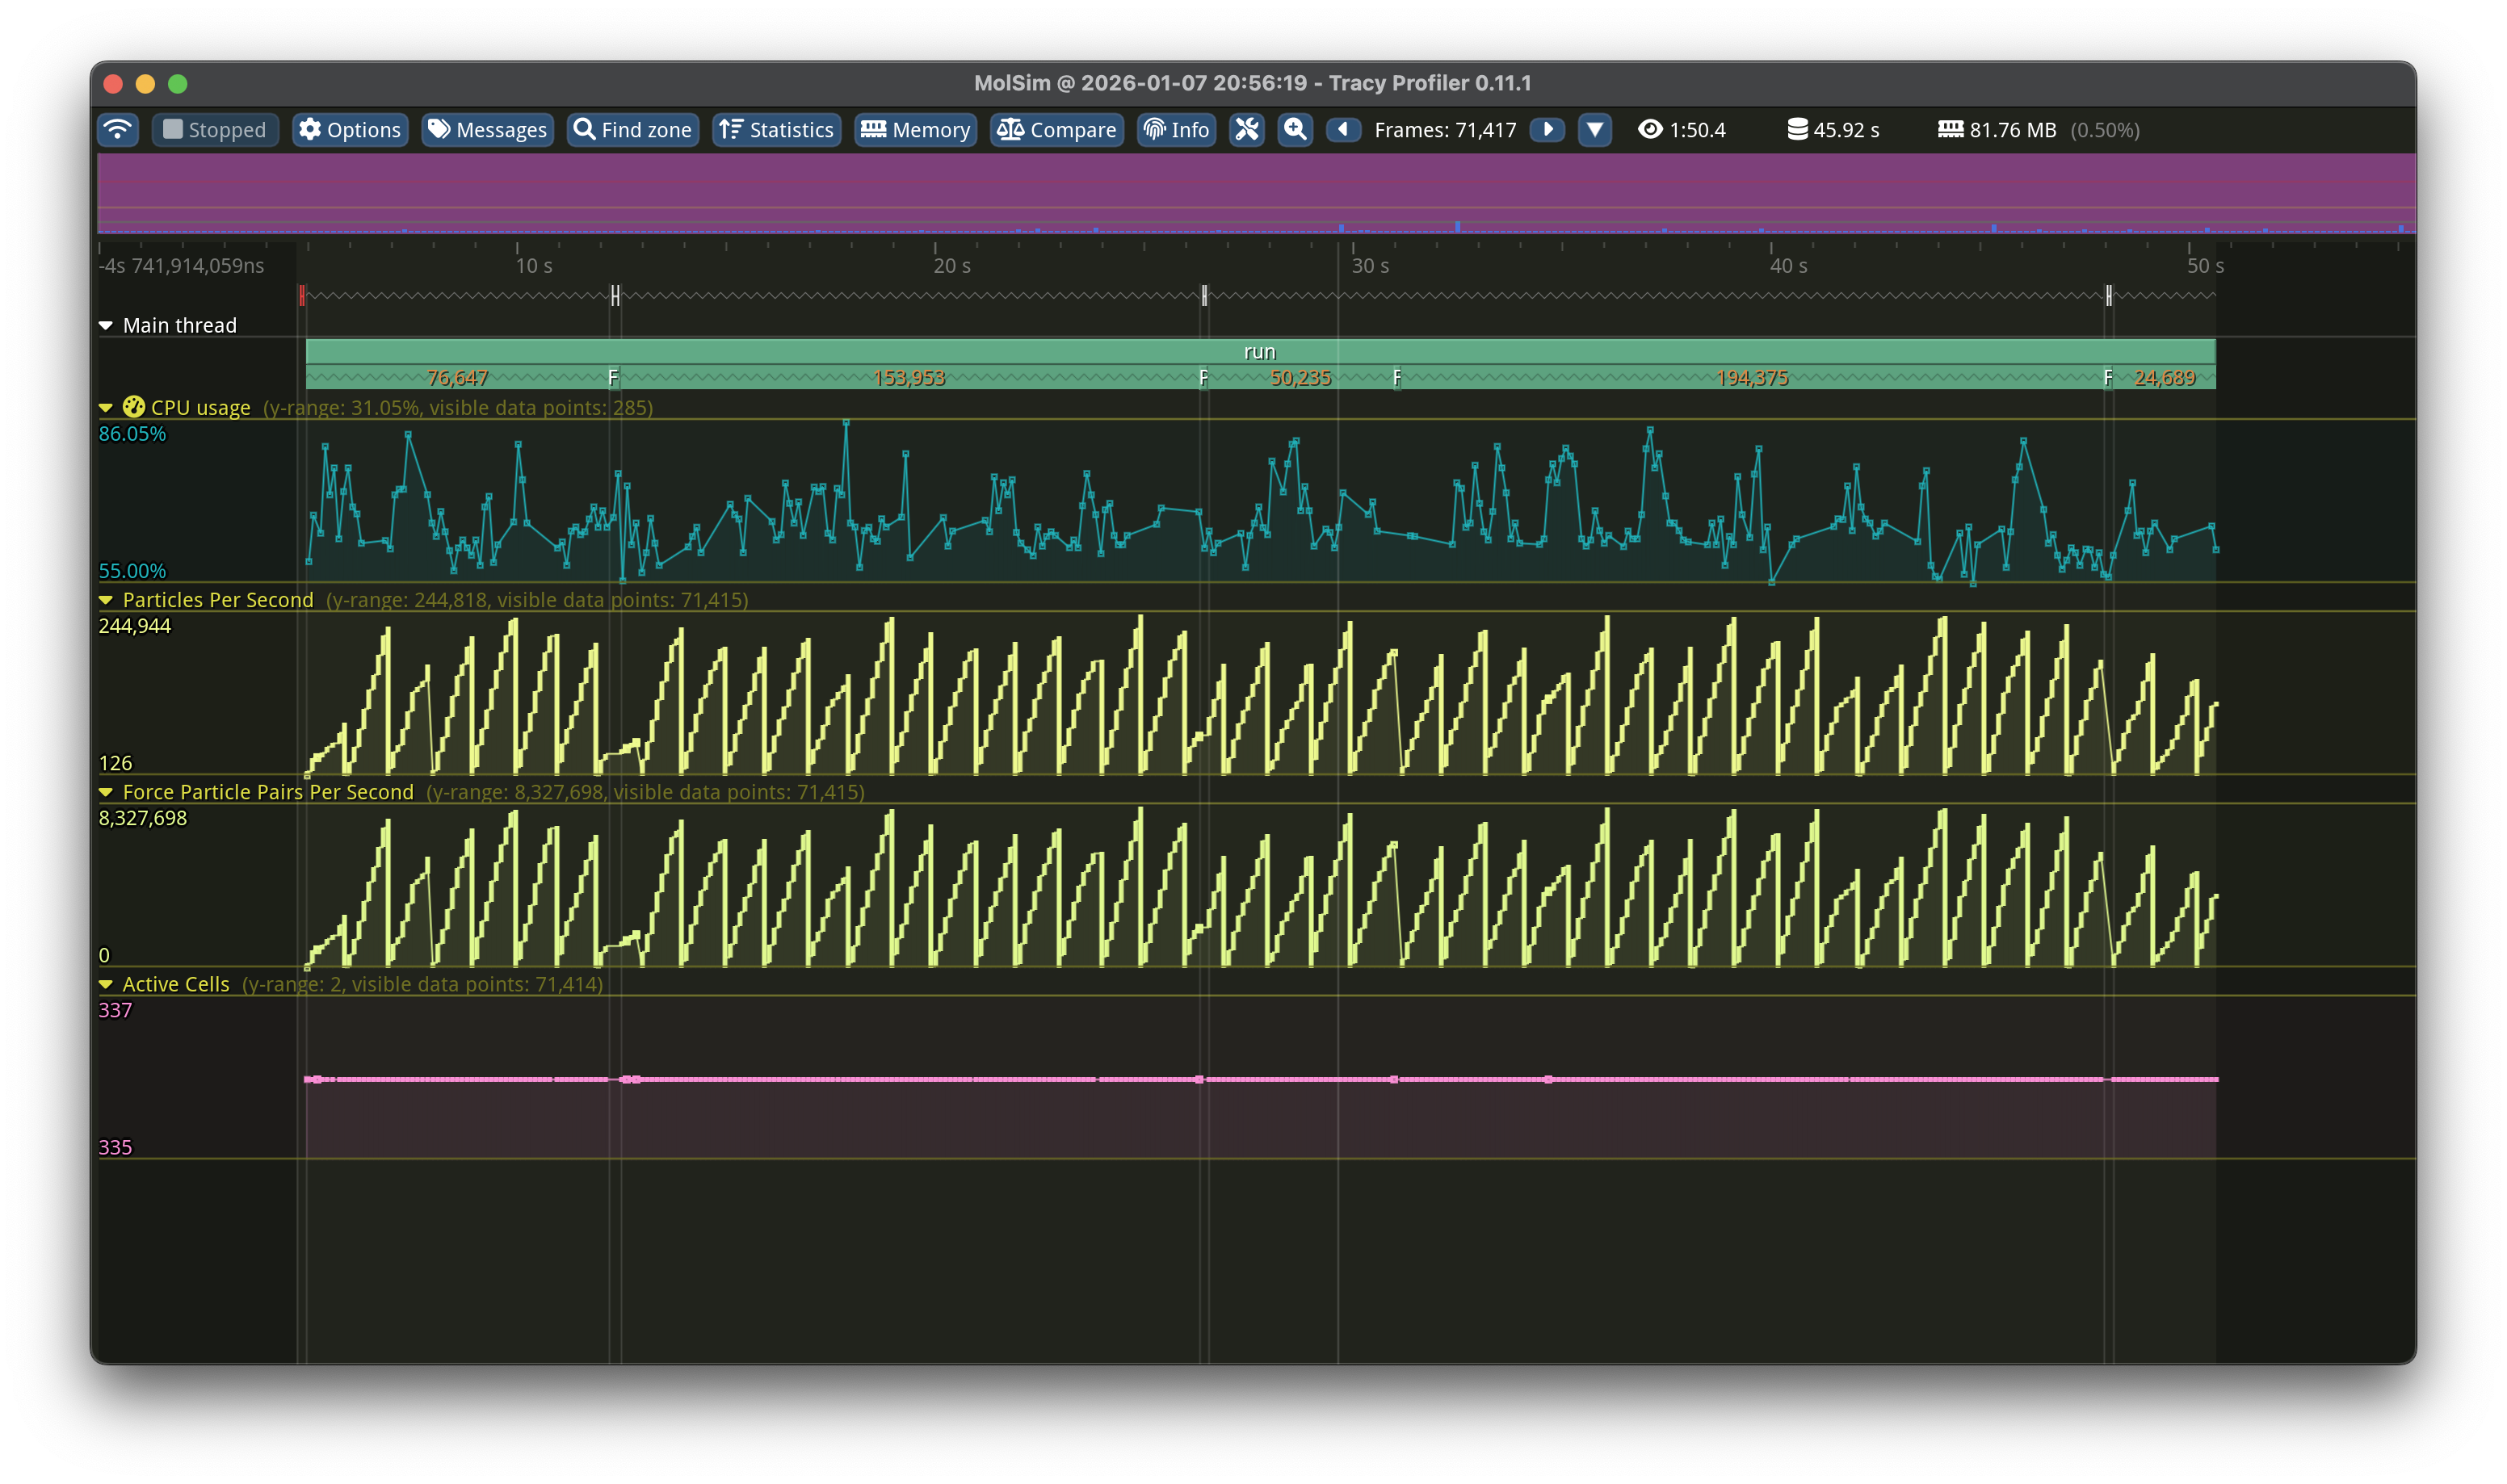
\includegraphics[width=0.85\textwidth]{media/profile-example.png}
                    \end{center}
    \end{frame}

    \simpleframe\begin{frame}[noframenumbering]{Profiling Integration}{Tracy Zones}
                    \begin{center}
                        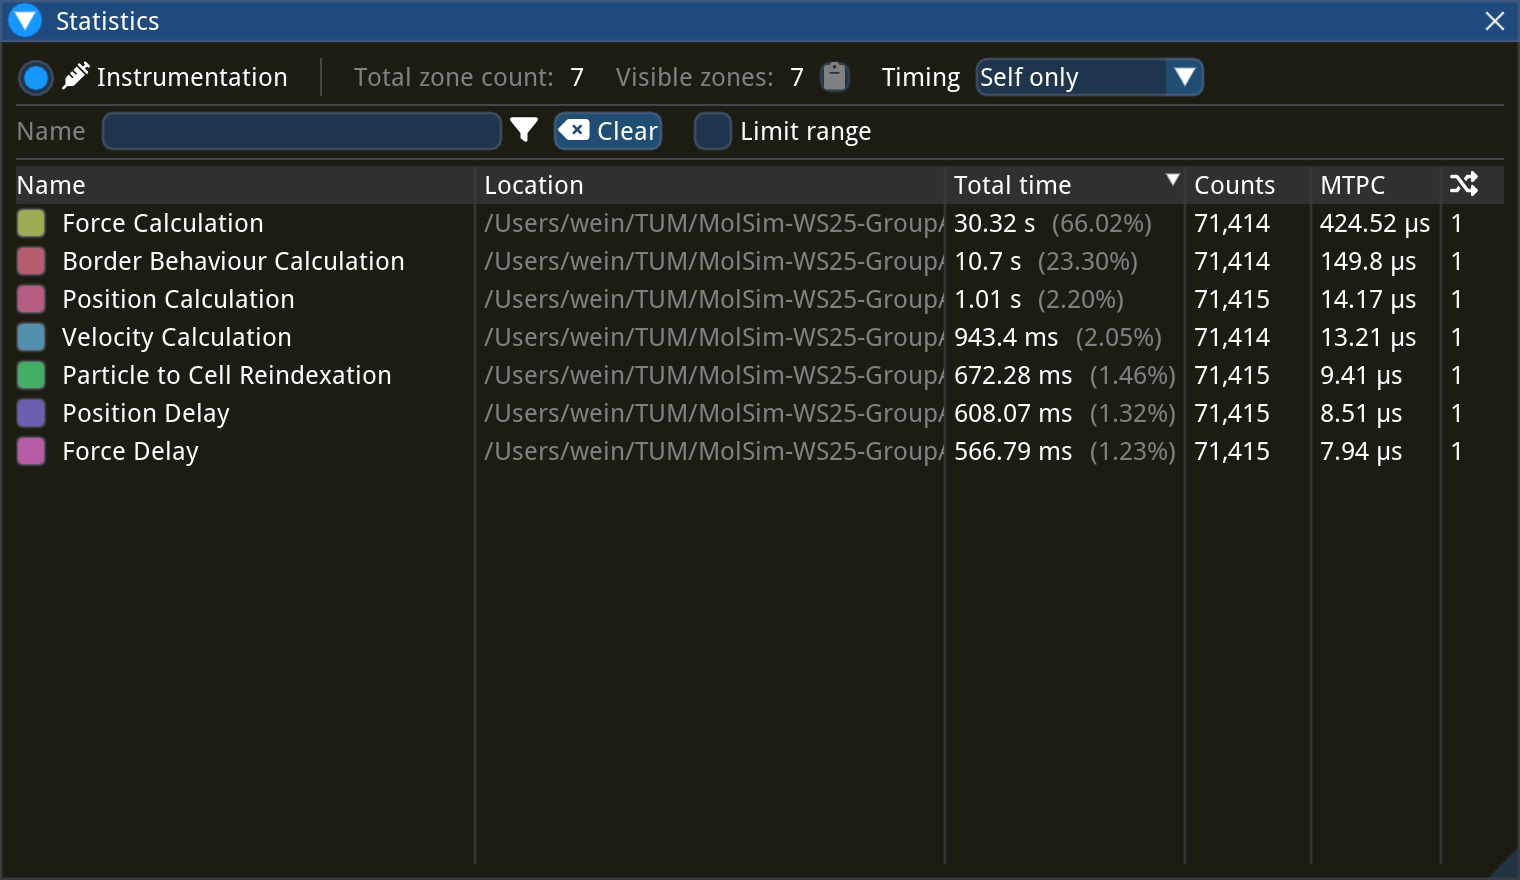
\includegraphics[width=0.5\textwidth]{media/profile-zones.png}
                    \end{center}

                    Position and Velocity updates are efficient, the most time-consuming part is border behaviour calculation as well as force calculation.\footnotemark

                    \blue{We need to focus on optimizing force calculation and border behaviour.}

                    \footnotetext[1]{Commit: cc4ed05a08ea63fc6138b524bb29cfacbb9d7409, running \texttt{./build/MolSim input/cuboid-3200.yml -t 10000 }}
    \end{frame}

    \simpleframe\begin{frame}{Profiling Integration}{Tracy Benefits}
                    \begin{itemize}
                        \item \blue{Nanosecond Resolution}: Extremely precise profiling.
                        \item \blue{Frame captures}: Analyze performance over simulation loops. \blue{Perfect for us!}
                        \item \blue{Custom Zones}: Profile specific code sections like force calculations.
                        \item \blue{Zero overhead when disabled!} Performance unaffected in release builds.
                    \end{itemize}
    \end{frame}

    \section{Task 3}

    \begin{frame}{Simulation Setup}
        \begin{itemize}
            \item Two-phase simulation:
            \begin{itemize}
                \item Equilibration run with thermostat ($t = 15$)
                \item Actual simulation with falling drop ($t = 40$)
            \end{itemize}
            \item Checkpoint written after equilibration
            \item Restart simulation from checkpoint and add a disc
        \end{itemize}
    \end{frame}

    \begin{frame}{Checkpointing}
        \begin{itemize}
            \item Implemented a checkpoint writer
            \item Stores complete phase space:
            \begin{itemize}
                \item Positions, velocities
                \item Forces and old forces
                \item Particle properties (mass, type, etc.)
            \end{itemize}
            \item Checkpoint file can be used as input for a new simulation
        \end{itemize}
    \end{frame}

    \begin{frame}{Visualization}
        \begin{frame}{Profiling Integration}
            \begin{center}
                \begin{minipage}{0.45\textwidth}
                    \includegraphics[width=\linewidth]{media/asm4task4.0.png}
                \end{minipage}
                \hfill
                \begin{minipage}{0.45\textwidth}
                    \includegraphics[width=\linewidth]{media/asm4task4.1.png}
                \end{minipage}

                \vspace{0.5em}

                \begin{minipage}{0.45\textwidth}
                    \includegraphics[width=\linewidth]{media/asm4task4.2.png}
                \end{minipage}
                \hfill
                \begin{minipage}{0.45\textwidth}
                    \includegraphics[width=\linewidth]{media/asm4task4.3.png}
                \end{minipage}
            \end{center}
        \end{frame}


        \vspace{0.3cm}
        {\footnotesize Visualization of the falling drop using OVITO(.xyz file is bit lighter than .vtk for massive particles).}
    \end{frame}

\end{frame}



\begin{frame}{Measurement Setup}
    \begin{itemize}
        \item Large representative scenario ($\geq$ 10,000 molecules)
        \item I/O disabled during measurements
        \item Measurements performed with compiler optimizations enabled
        \item Build type: \texttt{Release} (O3)
    \end{itemize}
\usebackgroundtemplate{\framebackground{0.2}{0}}
\begin{frame}
    \maketitle
\end{frame}

\simpleframe\begin{frame}{Thermostats}
\begin{center}
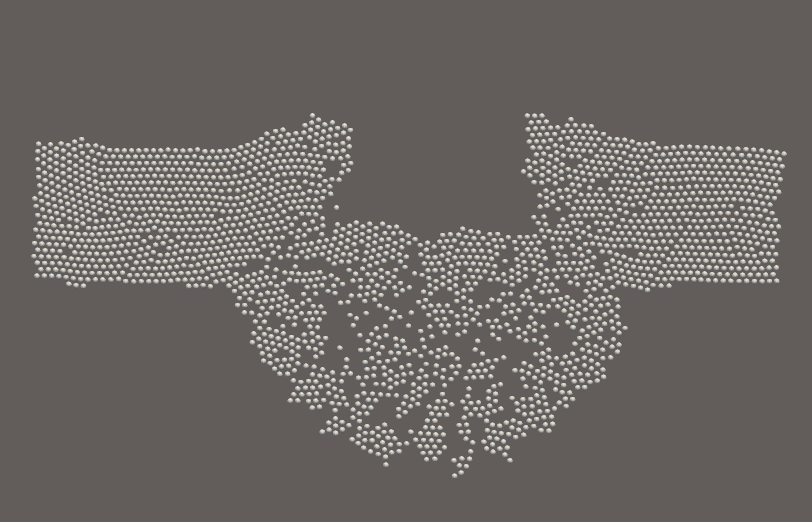
\includegraphics[width=0.6\textwidth]{media/lowTemp_2Bodies.png}
\end{center}
As seen in lowTemp2Bodies.mp4
\end{frame}

\simpleframe\begin{frame}{Thermostats}
\begin{center}
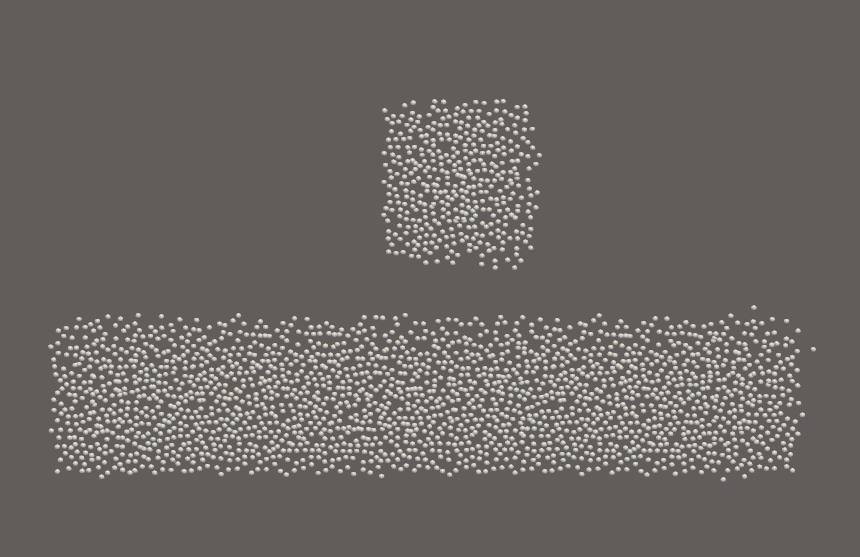
\includegraphics[width=0.6\textwidth]{media/highTemp_2Bodies.png}
\end{center}
As seen in highTemp2Bodies.mp4
\end{frame}

\simpleframe\begin{frame}{Problem with reflective boundaries}
\begin{center}
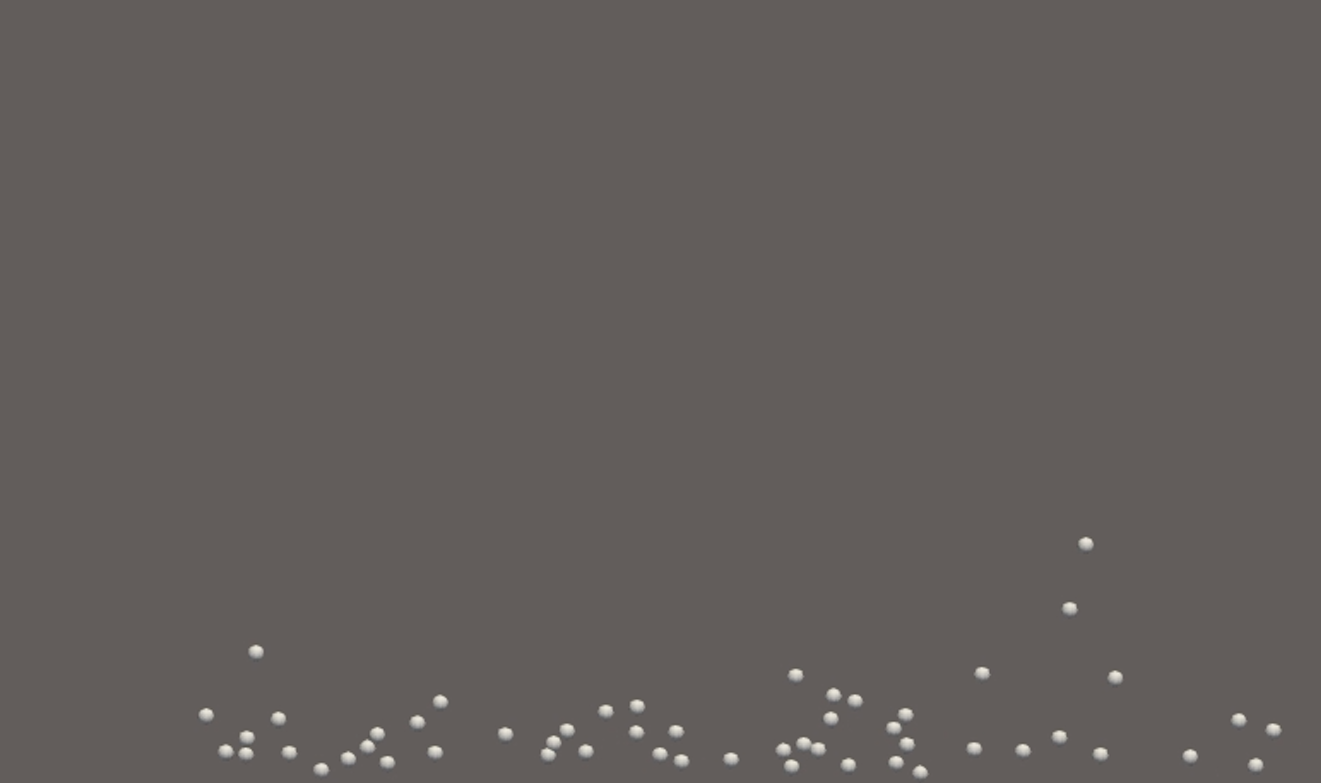
\includegraphics[width=0.60\textwidth]{media/normGrav.png}
\end{center}
A problem appears with balancing repulsion strength between wall and particles.

As seen in liquid2normGravity.mp4
\end{frame}

\simpleframe\begin{frame}{Problem with reflective boundaries}
\begin{center}
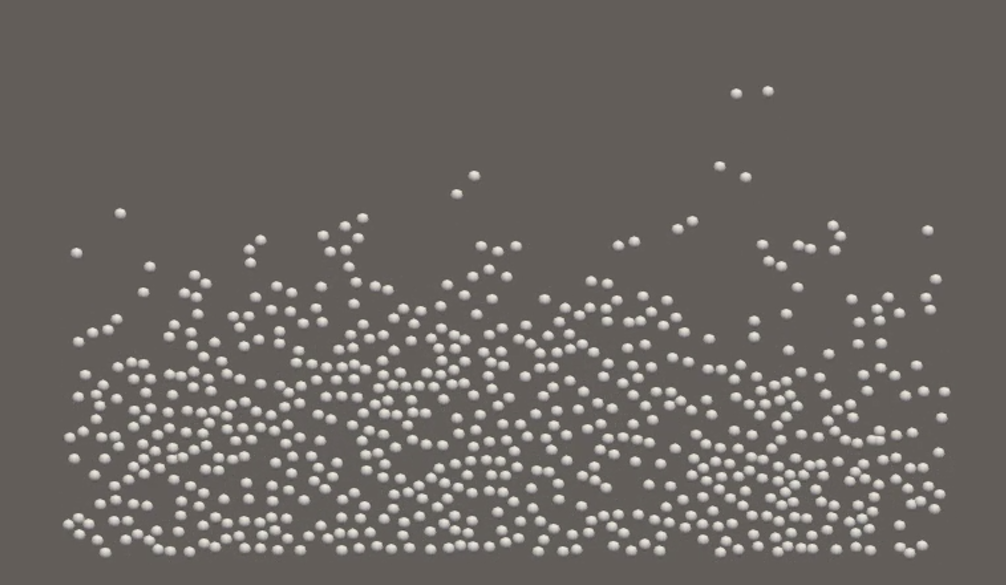
\includegraphics[width=0.60\textwidth]{media/lowGrav.png}
\end{center}
Solved by clamping particles back into domain space, resulting unnatural velocity behavior.
This is not ideal.
As seen in liquid2LowGravity.mp4
\end{frame}

\begin{frame}{Runtime Measurement}
    \begin{itemize}
        \item Windows 11 home 64bits
        \item Bios: E15K1IMS.114
        \item CPU: 13th Gen Intel(R) Core(TM) i7-13620H(16CPUs), 2.4GHz
        \item RAM: 16384MB
        \item Graphic: NVIDIA GeForce RTX 4060 Laptop GPU

    \end{itemize}
    \begin{center}
        \includegraphics[width=0.5\textwidth]{media/Runtime Measurement.png}
    \end{center}
\end{frame}

\begin{frame}{Profiling}
    \begin{itemize}
        \item Profiling performed using:
        \begin{itemize}
            \item gprof / perf ...
        \end{itemize}
        \item Profiling reveals most time spent in:
        \begin{itemize}
            \item Force calculation
            \item Neighbor traversal (Linked Cell)
        \end{itemize}
    \end{itemize}
\end{frame}


\section{Task 5}
\begin{frame}{Compiler Optimizations: gcc}
    \begin{table}[htbp]
        \centering

        \label{tab:perf_4x6}
        \setlength{\tabcolsep}{6pt}
        \renewcommand{\arraystretch}{1.5}

        \begin{tabular}{lrrrrrr}
            \toprule
            Method  & Runtime (s) & MUPS (M/s)  & Time/iteration (s)  \\
            \midrule
            Debug/Baseline & 92.739 & 0.0108 & 0.0092  \\
            RelDebInfo & 30.4273 & 0.0329 & 0.0031 \\
            Release & 28.2528 & 0.0354 & 0.0028 \\
            \bottomrule
        \end{tabular}
        \caption{Performance comparison (100 particles; 10000 times iterations)}
    \end{table}
\end{frame}

\begin{frame}{Compiler Optimizations: Clang}
    \begin{table}[htbp]
        \centering

        \label{tab:perf_4x6}
        \setlength{\tabcolsep}{6pt}
        \renewcommand{\arraystretch}{1.5}

        \begin{tabular}{lrrrrrr}
            \toprule
            Method  & Runtime (s) & MUPS (M/s)  & Time/iteration (s)  \\
            \midrule
            Debug/Baseline & 38.7201 & 0.0258 & 0.0039  \\
            Ofast & 38.8976 & 0.0257 & 0.0039 \\
            \bottomrule
        \end{tabular}
        \caption{Performance comparison (100 particles; 10000 times iterations)}
    \end{table}
\end{frame}


\begin{frame}{Algorithmic and Code-Level Optimizations}
    \begin{itemize}
        \item Use Linked Cell algorithm instead of direct summation
        \item Reduce unnecessary distance calculations
        \item Reuse previously computed values where possible
        \item Avoid unnecessary square root computations
        \item Inline small frequently used functions
        \item Improve data locality in particle containers
    \end{itemize}
    \begin{table}[htbp]
        \centering

        \label{tab:perf_4x6}
        \setlength{\tabcolsep}{6pt}
        \renewcommand{\arraystretch}{1.5}

        \begin{tabular}{lrrrrrr}
            \toprule
            Method  & Runtime (s) & MUPS (M/s)  & Time/iteration (s)  \\
            \midrule
            Baseline & 92.739 & 0.0108 & 0.0092  \\
            OpenMP & 34.5515 & 0.0289& 0.0035  \\
            \bottomrule
        \end{tabular}
        \caption{Algorithmic Optimizations with gcc (100 particles; 10000 times iterations)}
    \end{table}
\end{frame}

\begin{frame}{Compiler Optimizations}
    \begin{itemize}
        \item GCC with optimization level \texttt{-O3}
        \item Profile-Guided Optimization (PGO)
        \item Comparison with Intel LLVM compiler (\texttt{icpx})
    \end{itemize}
\end{frame}

\end{document}